\documentclass[UTF8]{ctexart}
\ctexset { section = { format={\Large \bfseries } } }
\pagestyle{plain}
\usepackage{float}
\usepackage{amsmath}
\usepackage{amssymb}
\usepackage{listings}
\usepackage{graphicx}%插入图片宏包
\usepackage{xcolor}
\usepackage{geometry}
\geometry{a4paper,scale=0.8}
\usepackage{caption}
\usepackage{subcaption}
\usepackage[colorlinks=true, linkcolor=blue, citecolor=blue, urlcolor=blue]{hyperref}
\captionsetup[figure]{name={Figure}}
\captionsetup[table]{name={Table}}
\usepackage{hyperref}
\definecolor{Rhodamine}{RGB}{227,11,92}


\lstset{
language=Python, % 设置语言
basicstyle=\ttfamily\small, % 设置字体族
breaklines=true, % 自动换行
keywordstyle=\bfseries\color{blue}, % 设置关键字为粗体,
morekeywords={}, % 设置更多的关键字,用逗号分隔
emph={self}, % 指定强调词,如果有多个,用逗号隔开
emphstyle=\bfseries\color{Rhodamine}, % 强调词样式设置
commentstyle=\color{black!50!white}, % 设置注释样式,斜体,浅灰色
stringstyle=\bfseries\color{red!90!black}, % 设置字符串样式
columns=flexible,
numbers=left, % 显示行号在左边
numbersep=2em, % 设置行号的具体位置
numberstyle=\footnotesize, % 缩小行号
frame=single, % 边框
framesep=1em % 设置代码与边框的距离
}

\title{\textbf{Image Processing Homework 5}}
\author{吴嘉骜 21307130203}
\date{\today}

\begin{document}

\maketitle

\noindent
\section{}
\setlength{\parindent}{0pt}
Implement the generation of noise.\\
For images of the brain, heart (or other images), generate the following 
two different types of noise with varying intensities:\\
(1) Generate white noise;\\
(2) Generate another type of noise (such as Gaussian, Rayleigh, or salt-and-pepper noise).\\
Contaminate the images with the generated noise and visually compare the images before and after the noise pollution.\\
\textbf{Solution}:\\
The code from \texttt{noisegen.py} is shown as follows.\\
\begin{lstlisting}
from PIL import Image
import numpy as np
import matplotlib.pyplot as plt
from numpy.fft import fft2, ifft2, fftshift, ifftshift
...
# Auxiliary functions are descibed below and omitted here.
def white_noise_gen(shape, amplitude):
    '''
    Generate white noise.
    
    Parameters:
        - shape: the size of the noise, a tuple of (height, width).
        - spectrum: the spectrum of the noise, a constant.
    Returns:
        - noise: the generated noise, a numpy array.
    '''
    f = np.full(shape, amplitude)  # generate constant spectrum
    u0, v0 = (shape[0]//2, shape[1]//2)  # get the center of the spectrum
    
    phase = np.exp(2j * np.pi * np.random.random(shape))  # generate random phase
    f = f * phase  # generate half of the noise spectrum
    for i in range(u0+1, shape[0]):
        for j in range(shape[1]):
            if 0 <= 2*u0-i <= 255 and 0 <= 2*v0-j <= 255:
                f[i][j] = np.conj(f[2*u0-i][2*v0-j])
    f[u0, v0] = amplitude  # set the center of the spectrum to real
    noise = np.real(ifft2(ifftshift(f)))  # generate white noise in the spatial domain
    
    return noise

def gaussian_noise_gen(shape, mean, std):
    '''
    Generate gaussian noise.
    
    Parameters:
        - shape: the size of the noise, a tuple of (height, width).
        - mean: the mean of the gaussian distribution.
        - std: the standard deviation of the gaussian distribution.
    Returns:
        - noise: the generated noise, a numpy array.
    '''
    noise = np.random.normal(mean, std, shape)  # generate gaussian random number
    return noise

def rayleigh_noise_gen(shape, a, b):
    '''
    Generate raleigh noise.
    
    Parameters:
        - shape: the size of the noise, a tuple of (height, width).
        - a, b: parameters of the rayleigh distribution.
    Returns:
        - noise: the generated noise, a numpy array.
    '''
    u = np.random.uniform(0, 1, shape)  # generate uniform random number
    noise = a + np.sqrt(-b * np.log(1 - u))  # inverse transform sampling
    return noise

def img_interfere(img, noise=None, s_p=0 , ps=0, pp=0):
    '''
    Interfere the image with the noise.
    
    Parameters:
        - img: the image to be interfered, a numpy array.
        - noise: the noise to interfere the image, a numpy array. For salt and pepper noise, the input noise is None.
        - s_p: a flag to indicate whether the noise is salt and pepper noise. 0 for no, 1 for yes.
        - ps: the probability of salt noise.
        - pp: the probability of pepper noise.
    Returns:
        - img_interfered: the interfered image, a numpy array.
    '''
    if s_p ==0:
        img_interfered = img + noise
        return img_interfered
    else:
        # salt and pepper noise
        img_interfered = img.copy()
        for i in range(img.shape[0]):
            for j in range(img.shape[1]):
                if np.random.random() < ps:
                    img_interfered[i][j] = 255
                elif np.random.random() < pp:
                    img_interfered[i][j] = 0
        return img_interfered
\end{lstlisting}
We first interpret the code structure briefly, and later we will explain the key functions in detail.

\textbf{read\_img}: Reads an image from the given path and converts it to a grayscale numpy array.

\textbf{show\_image}: Displays the image using matplotlib with specified figure size and colormap.

\textbf{img\_modify}: Normalizes and processes the image for display based on the specified modification type, including logarithmic transformation, clipping, and scaling.

\textbf{show\_spectrum}: Computes and displays the frequency spectrum of the image.

\textbf{show\_spectrum2}: Displays the frequency spectrum from a given discrete Fourier transform (DFT).

\textbf{white\_noise\_gen}: Generates white noise with the specified shape and amplitude.

\textbf{gaussian\_noise\_gen}: Generates Gaussian noise with the specified shape, mean, and standard deviation.

\textbf{rayleigh\_noise\_gen}: Generates Rayleigh noise with the specified shape, location parameter, and scale parameter.

\textbf{img\_interfere}: Interferes the image with the specified noise, including salt-and-pepper noise.

\textbf{Details}:\\
For white noise, we generate a constant spectrum, and then apply a random phase spectrum to it. To ensure the noise in the spatial domain is real, we set the frequency domain conjugate symmetric.\\
For Gaussian noise, we directly generate normal distribution random numbers by \texttt{np.random.normal}.\\
For Rayleigh noise, we generate random numbers by the inverse transform method. Note tbar the cumulative distribution function of Rayleigh distribution is
$F(z;a,b)=1-e^{-\frac{(z-a)^2}{2b^2}}$, where $a$ is the location parameter and $b$ is the scale parameter. Let $u$ be a uniform random variable in $[0,1]$, then $F^{-1}(u;a,b)=a+b\sqrt{-2\ln(1-u)}$.
Thus, we can generate Rayleigh distribution random numbers by applying $F^{-1}$ to uniform random numbers.\\
Above three noises can be added to the image simply. For salt-and-pepper noise, however, we determine the polluting probability by comparing $u$ with a preset threshold $p$, and directly interfere the image with it.\\
\textbf{Results}:\\
The results are presented in Figure \ref{fig:brain} and Figure \ref{fig:heart}.\\
\begin{figure}[htbp]
    \centering
    \begin{subfigure}{0.3\textwidth}
        \centering
        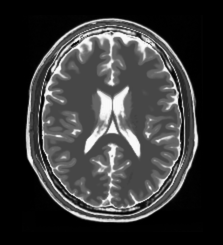
\includegraphics[width=\linewidth]{brainimg.png}
        \caption{Original image}
    \end{subfigure}%
    \hfill
    \begin{subfigure}{0.3\textwidth}
        \centering
        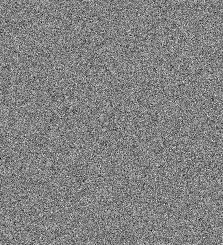
\includegraphics[width=\linewidth]{white_noise1.png}
        \caption{White noise spectrum $A=100$}
    \end{subfigure}%
    \hfill
    \begin{subfigure}{0.3\textwidth}
        \centering
        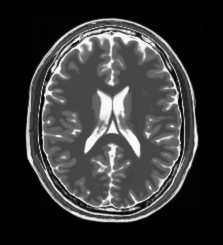
\includegraphics[width=\linewidth]{brain_noised_white.png}
        \caption{White noise pollution}
    \end{subfigure}

    \vspace{0.5cm}
    \centering
    \begin{subfigure}{0.3\textwidth}
        \centering
        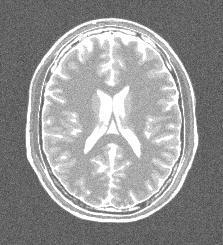
\includegraphics[width=\linewidth]{brain_noised_gaussian.png}
        \caption{Gaussian noise pollution, $\mu=100$, $\sigma=10$}
    \end{subfigure}%
    \hfill
    \begin{subfigure}{0.3\textwidth}
        \centering
        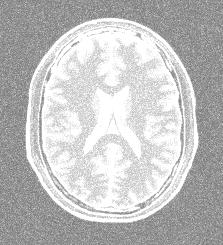
\includegraphics[width=\linewidth]{brain_noised_rayleigh.png}
        \caption{Rayleigh noise pollution, $a=120$, $b=1000$}
    \end{subfigure}%
    \hfill
    \begin{subfigure}{0.3\textwidth}
        \centering
        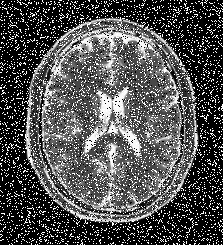
\includegraphics[width=\linewidth]{brain_noised_s_p.png}
        \caption{Salt-and-pepper noise pollution, $p_s=0.15$, $p_p=0.08$}
    \end{subfigure}
    \caption{Brain image after noise pollution}
    \label{fig:brain}
\end{figure}

\begin{figure}[htbp]
    \centering
    \begin{subfigure}{0.3\textwidth}
        \centering
        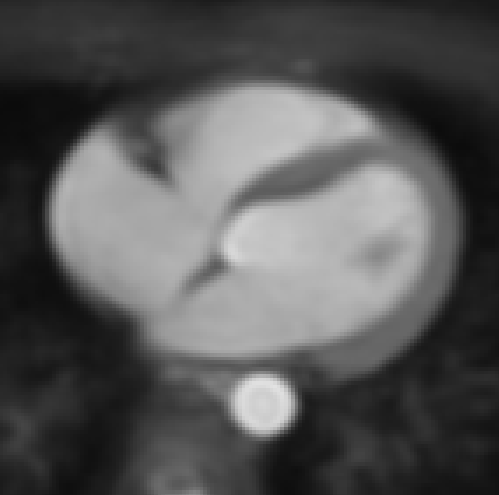
\includegraphics[width=\linewidth]{heartimg.png}
        \caption{Original image}
    \end{subfigure}%
    \hfill
    \begin{subfigure}{0.3\textwidth}
        \centering
        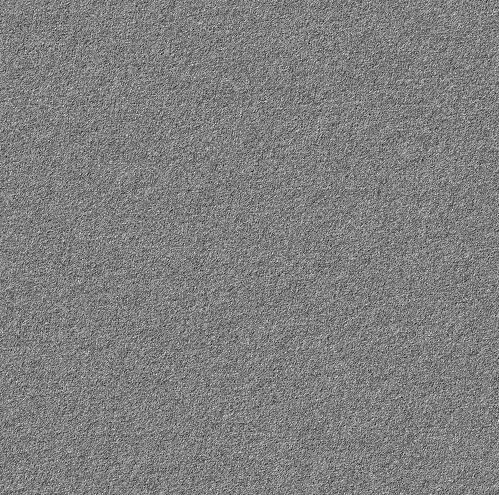
\includegraphics[width=\linewidth]{white_noise2.png}
        \caption{White noise spectrum $A=200$}
    \end{subfigure}%
    \hfill
    \begin{subfigure}{0.3\textwidth}
        \centering
        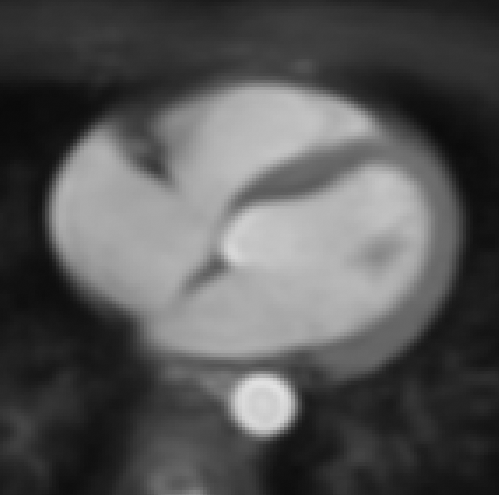
\includegraphics[width=\linewidth]{heart_noised_white.png}
        \caption{White noise pollution}
    \end{subfigure}

    \vspace{0.5cm}
    \centering
    \begin{subfigure}{0.3\textwidth}
        \centering
        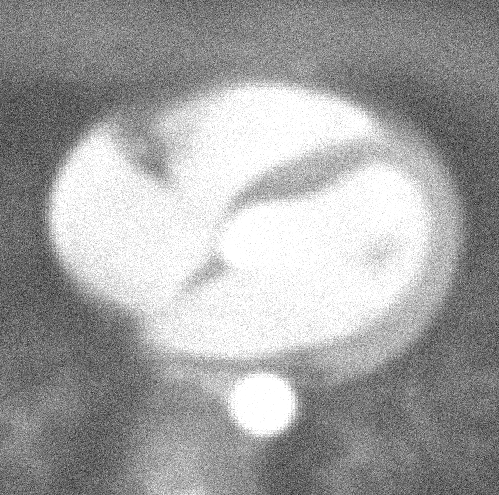
\includegraphics[width=\linewidth]{heart_noised_gaussian.png}
        \caption{Gaussian noise pollution, $\mu=80$, $\sigma=20$}
    \end{subfigure}%
    \hfill
    \begin{subfigure}{0.3\textwidth}
        \centering
        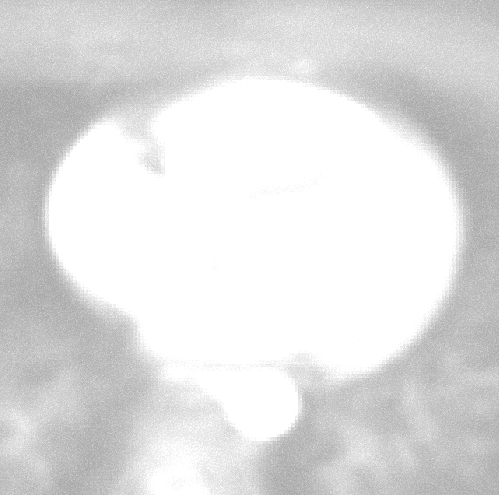
\includegraphics[width=\linewidth]{heart_noised_rayleigh.png}
        \caption{Rayleigh noise pollution, $a=150$, $b=200$}
    \end{subfigure}%
    \hfill
    \begin{subfigure}{0.3\textwidth}
        \centering
        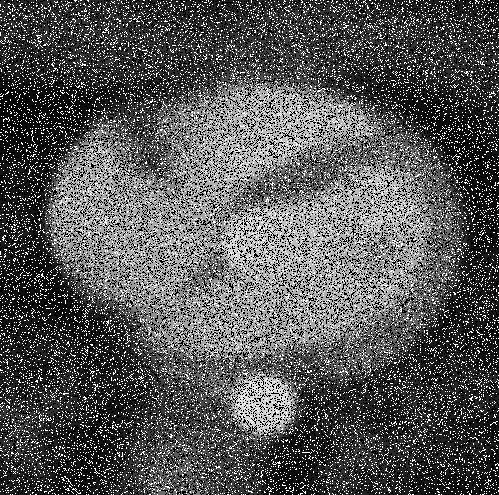
\includegraphics[width=\linewidth]{heart_noised_s_p.png}
        \caption{Salt-and-pepper noise pollution, $p_s=0.13$, $p_p=0.27$}
    \end{subfigure}
    \caption{Heart image after noise pollution}
    \label{fig:heart}
\end{figure}
\textbf{Analysis}:\\
White noise is hard to observe visually in the polluted image, but it can be seen from the spectrum tbar the noise is evenly distributed in the frequency domain. 

Gaussian noise is characterized by the mean and standard deviation, which determine the brightness and the intensity range, respectively. Both polluted images 
are blurred and brighter than the original image.

Rayleigh noise is characterized by parameters $a$ and $b$, which determine the shift in the brightness and the probability of the noise, respectively. The effect is similar to Gaussian noise.

For salt-and-pepper noise, It is observable tbar the larger the probability of salt noise, the brighter the noise points, and the larger the probability of pepper noise, the darker the noise points.

\newpage
\section{}
Implement an optimal notch filter, and test its effect with images.\\
\textbf{Solution}:\\
The code from \texttt{opt\_nf.py} is shown as follows.\\

\begin{lstlisting}
from PIL import Image
import numpy as np
import matplotlib.pyplot as plt
...
# Auxiliary functions are the same as noisegen.py, and omitted here.
def ghpf_shift(img, d0, u0, v0):
    '''
    Gaussian high pass filter (GHPF) with center shifted to (u0, v0).
    
    Parameters:
        - img: the input image, a 2D numpy array
        - d0: the cutoff frequency
        - u0, v0: the center coordinates of the highpass filter
        
    Returns:
        - filter_transfun: the filter transfer function of GHPF, with size m*n
    '''
    m, n = img.shape
    filter_transfun = np.zeros((m, n))
    for u in range(m):
        for v in range(n):
            d2 = (u-u0)**2 + (v-v0)**2
            filter_transfun[u, v] = 1 - np.exp(-d2/(2*d0**2))
    return filter_transfun

def notch_reject(img, coord, d0):
    '''
    Notch reject filter.
    
    Parameters:
        - img: the input image, a 2D numpy array
        - coord: the center coordinates of each highpass filter, k*2 array, k is the number of filters
        - d0: the cutoff frequency of the highpass filter
        
    Returns:
        - filter_transfun: the filter transfer function of notch reject filter, with size m*n
    '''
    m, n = img.shape
    k = coord.shape[0]
    nr = np.ones((m,n))
    for i in range(k):
        u, v = coord[i]
        nr *= ghpf_shift(img, d0, u, v) * ghpf_shift(img, d0, m-u, n-v)
    return nr

def notch_pass(img, coord, d0):
    '''
    Notch pass filter.
    '''
    return 1-notch_reject(img, coord, d0)

def optimum_notch(img, notch, m1, n1):
    '''
    Optimum notch filter.
    
    Parameters:
        - img: the input image, a 2D numpy array
        - notch: the notch filter transfer function, the same size as img
        - m1, n1: the size of the neighborhood, two odd integers
        
    returns:
        - img_filtered: the filtered image, a 2D numpy array
    '''
    def meanvalue(img, x, y, m1, n1):
        '''
        Calculate the mean value of the neighborhood of each pixel.
        - x,y: the center coordinates of the neighborhood
        '''
        m, n = img.shape
        img_mean = 0
        i1 = max(0, x-m1//2)
        i2 = min(m, x+m1//2+1)
        j1 = max(0, y-n1//2)
        j2 = min(n, y+n1//2+1)
        img_mean = np.mean(img[i1:i2, j1:j2])
        return img_mean
    
    m, n = img.shape
    w = np.zeros((m, n))
    
    # DFT of the image
    fg = np.fft.fft2(img)
    fg = np.fft.fftshift(fg)
    
    # interference pattern in sptaial domain
    eta = fg * notch
    eta = np.fft.ifftshift(eta)  
    eta = np.fft.ifft2(eta)
    eta = np.real(eta)
    
    # weighting function
    for x in range(m):
        for y in range(n):
            eta_bar = meanvalue(eta, x, y, m1, n1)
            eta2_bar = meanvalue(eta**2, x, y, m1, n1)
            geta_bar = meanvalue(img*eta, x, y, m1, n1)
            g_bareta_bar = meanvalue(img, x, y, m1, n1)*eta_bar
            w[x, y] = (geta_bar - g_bareta_bar) / (eta2_bar - eta_bar**2)
    
    # estimated f
    img_filtered = img - w * eta
    
    return img_filtered

# test
img_path = './noisy_image.png'
img = read_img(img_path)
m, n = img.shape
show_spectrum(img)

# create the filter transfer function
ys = np.arange(100, 37, -9)
xs = np.arange(105, -14, -17)
coor = np.column_stack((xs, ys))  # coordinates of bursts
k = coor.shape[0]
nr = np.ones((m,n))
for i in range(k):
    u, v = coor[i]
    nr *= ghpf_shift(img, 4.5, u, v) * ghpf_shift(img, 4.5, m-u, n-v)
nr *= ghpf_shift(img, 2, 137.8, 85) * ghpf_shift(img, 2, m-137.8, n-85)
notch = 1 - nr

img_filtered = optimum_notch(img, notch, 7, 5)
img_out = img_modify(img_filtered, modified=2)
show_spectrum(img_out)
show_image(img_out)
\end{lstlisting}
The key function is \texttt{optimum\_notch}, which implements the optimum notch filter. It receives the image,
a notch filter transfer function, and the size of the neighborhood as input, and returns the filtered image.\\
Inside, we define a function \texttt{meanvalue} to calculate the mean value of the neighborhood of each pixel, carefully
considering the boundary conditions. Then we calculate the DFT of the image $g$, and multiply it with the notch filter transfer function. After inverse DFT, we get the interference pattern $\eta$ in the spatial domain. 
Then we calculate the weighting function $w$ by the formula $\frac{\overline{g\eta}-\bar{g}\bar{\eta}}{\overline{\eta^2}-\bar{\eta}^2}$ for each $(x,y)$,
and the estimated image $f$ is obtained by $f=g-w\eta$.\\

\textbf{Test and Results}:\\
For testing, we manually pollute the brain image with peroidic noise, and then apply the optimum notch filter to it. 
We generate a noise pattern by superimposing multiple sine and cosine waves with varying frequencies and amplitudes. 
This pattern is then rotated to create a diagonal effect and added to the clean brain image, as shown in Figure \ref{fig:brain1}(b).
To construct a notch filter transfer function, we estimate the locations of the bursts by visual inspection and mouse hovering on the spectrum.
The parameters such as $d_0$ in GHPF and the window size are determined after several trials.
Then we use shifted Gaussian high pass filters product as input to formulate our optimum notch filter. The processed spectrum and estimated image are
also presented below.\\
\begin{figure}[htbp]
    \centering
    \begin{subfigure}{0.3\textwidth}
        \centering
        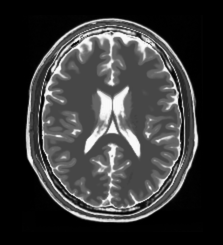
\includegraphics[width=\linewidth]{brainimg.png}
        \caption{Original image}
    \end{subfigure}%
    \hfill
    \begin{subfigure}{0.3\textwidth}
        \centering
        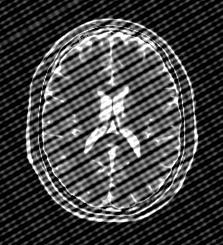
\includegraphics[width=\linewidth]{noisy_image.png}
        \caption{Image after noise pollution}
    \end{subfigure}%
    \hfill
    \begin{subfigure}{0.3\textwidth}
        \centering
        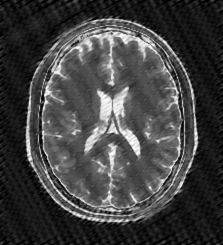
\includegraphics[width=\linewidth]{brain_cleaned.png}
        \caption{Processed image}
    
    \end{subfigure}

    \vspace{0.5cm}
    \centering
    \begin{subfigure}{0.5\textwidth}
        \centering
        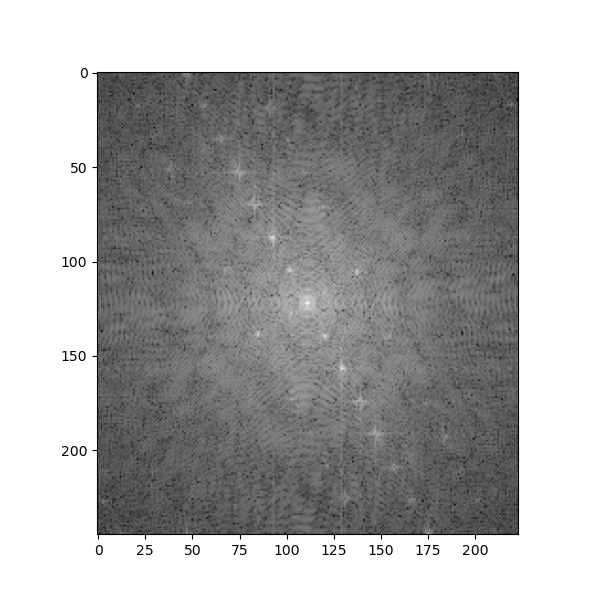
\includegraphics[width=1\linewidth]{spectrum_noised.png}
        \caption{Spectrum of polluted image}
    \end{subfigure}%
    \hfill
    \begin{subfigure}{0.5\textwidth}
        \centering
        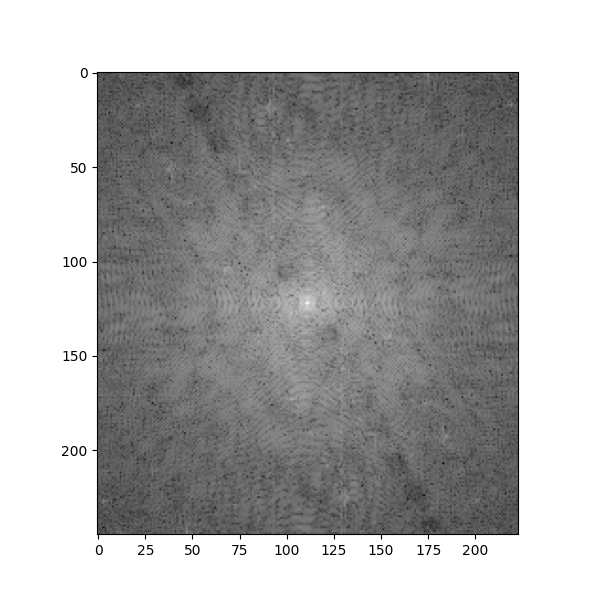
\includegraphics[width=\linewidth]{spectrum_cleaned.png}
        \caption{Filtered spectrum}
    \end{subfigure}%
    \caption{Optimum notch filter test}
    \label{fig:brain1}
\end{figure}

\textbf{Analysis}:\\
From the result, we observe that the spikes in the spectrum have been filtered out, and the
evident, disturbing stripe noises are removed. However, examining seriously, we still notice 
some artifacts in the background and the image boundary. The image is also slightly blurred, with some details within
the brain not clear as before.
We may perform smoothing and sharpening in further work to get a more satisfactory result.

\end{document}